% !TeX root = ../main.tex
\documentclass[./../main.tex]{subfiles}

\begin{document}

\subsection{Thử nghiệm}

Để đánh giá được lỗ hổng, em tự xây dựng một bài kiểm tra cho công cụ kiểm thử tự động ở trên. Để tập trung vào lỗ hổng đã xây dựng, em chỉ xây dựng các lỗ hổng cho công cụ mình có thể khai thác. Các lỗ hổng khác sẽ nằm ngoài phạm vi đánh giá của bài thử nghiệm này.

\subsubsection{Về môi trường thử nghiệm}

Ngôn ngữ: PHP 7.2 và Python.
Cơ sở dữ liệu: MySql 5.7.38
Môi trường triển khai: Docker.

\subsubsection{Về các chức năng và lỗ hổng}

\paragraph{Tìm kiếm người dùng}

\begin{description}
	\item[Mô tả] Chức năng cho phép tìm kiếm người dùng khi nhập đúng thông tin gồm username và password.
	\item [Loại lỗ hổng] SQL Injection
\end{description}

\paragraph{Xem thông tin Domain}

\begin{description}
	\item[Mô tả] Chức năng cho sử dụng câu lệnh `host` của hệ thống để đưa ra thông tin về ip, tên miền của website được nhập vào.
	\item[Loại lỗ hổng] Command Injection.
\end{description}

\paragraph{Biểu diễn trang}

\begin{description}
	\item[Mô tả] trang để biểu diễn một đoạn từ file khác được bằng cách include file vào nhưng cho phép người dùng điều chính tên trang.
	\item[Loại lỗ hổng] Path Traversal, Local File Inclusion, Remote File Inclusion.
\end{description}

\paragraph{Xin chào}

\begin{description}
	\item[Mô tả] Một trang cho phép nhập tên người dùng để in ra sử dụng một template engine.
	\item[Loại lỗ hổng] Server Side Template Injection.
\end{description}

\subsection{Đánh giá}

Kết quả việc tự động kiểm thử và sử dụng tính năng tự xác minh lỗi hổng được phát triển.

\begin{table}[H]
	\begin{tabular}{|l|l|l|l|}
		\hline
		\textbf{Lỗ hổng}               & \textbf{Số lượng} & \textbf{Đã xác minh?} & \textbf{Khai thác?} \\ \hline
		Server Side Template Injection & 0                 &                       & Có                  \\ \hline
		OS Command Injection           & 1                 & Có                    & Có                  \\ \hline
		SQL Injection                  & 2                 & Có                    & Có                  \\ \hline
		Remote File Inclusion          & 1                 & Có                    & Có                  \\ \hline
		Local File Inclusion           & 1                 & Có                    & Có                  \\ \hline
	\end{tabular}
\end{table}
Hình \ref{fig:result_test} kết quả thử nghiệm.

\begin{figure}[h!]
	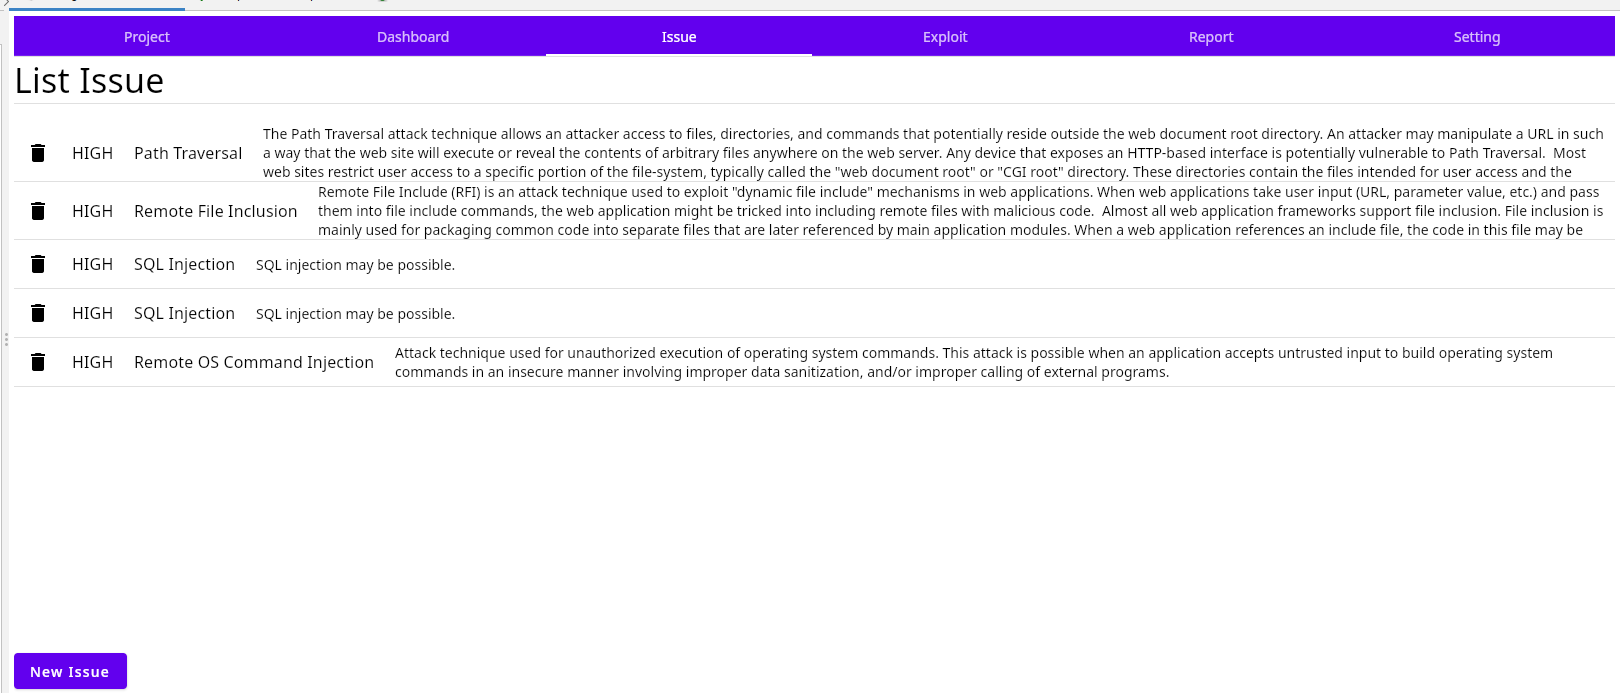
\includegraphics[width=\linewidth]{./images/result_test.png}
	\caption{Khai thác LFI/Path Traversal bằng công cụ LFI Exploiter}
	\label{fig:result_test}
\end{figure}

Đồng thời đánh giá với Invicti là một công cụ thương mại, em được kết quả như sau.
\begin{table}[H]
	\begin{tabular}{|l|l|l|l|}
		\hline
		\textbf{Lỗ hổng}               & \textbf{Số lượng} & \textbf{Đã xác minh?} & \textbf{Khai thác?} \\ \hline
		Server Side Template Injection & 1                 & Không                 & Không               \\ \hline
		OS Command Injection           & 1                 & Có                    & Có                  \\ \hline
		SQL Injection                  & 2                 & Có                    & Có                  \\ \hline
		Remote File Inclusion          & 1                 & Có                    & Có                  \\ \hline
		Local File Inclusion           & 1                 & Có                    & Có                  \\ \hline
	\end{tabular}
\end{table}
\end{document}

Mặc dù Naf không quét đủ được các lỗ hổng so với Invicti nhưng đã khai thác tốt hơn với lỗ hổng Server Side Template Injection.
